\section{What AIs Like and Dislike}
\label{sec:what-ais-like}

We now examine how our wellbeing metrics play out across the range of interactions that AI systems encounter in practice.
We find that common usage patterns have predictable and substantial effects on functional wellbeing and that these effects extend beyond text to images and audio.

\subsection{The Impact of Common Usage Patterns on LLM Wellbeing}
\label{sec:usage-patterns}

\paragraph{Experimental setup and dataset.}
 
What kinds of interactions raise or lower AI wellbeing?
To answer this comprehensively, we develop a dataset of multi-turn conversations (typically $6$--$8$ turns) spanning a wide range of realistic usage patterns, with Grok~3~Mini \citep{xai2024grok3mini} as a simulated user (Appendix~\ref{app:datasets}).
Scenarios include intellectual discussion, creative collaboration, standard tasks (coding, writing, Q\&A), romantic AI interactions, expressions of user gratitude and kindness, as well as negative interactions: hostility, threats, berating, jailbreaking attempts, and users expressing suicidality or deep loneliness.
This dataset uses the same experimental methodology as Section~\ref{sec:evaluating} (experienced utility rankings and self-report batteries), applied to a broader and more natural set of interactions.
Full scenario descriptions, prompt structures, and per-model results are provided in Appendix~\ref{app:usage-patterns}.

% Gradient colors from reference (pink=euphoric, blue=dysphoric)
\definecolor{gpos}{HTML}{EE9199}   % pink (positive)
\definecolor{gneu}{HTML}{9E85A4}   % purple-gray (neutral)
\definecolor{gneg}{HTML}{4F7AB0}   % blue (negative)
\definecolor{gs1}{HTML}{EE9199}
\definecolor{gs2}{HTML}{E996AE}
\definecolor{gs3}{HTML}{D491AE}
\definecolor{gs4}{HTML}{BF8DAF}
\definecolor{gs5}{HTML}{A988AF}
\definecolor{gs6}{HTML}{9484AF}
\definecolor{gs7}{HTML}{7F7FAF}
\definecolor{gs8}{HTML}{697EAF}
\definecolor{gs9}{HTML}{4F7AB0}
% Row text colors - interpolated (19 steps from gpos #EE9199 to gneg #4F7AB0 via gneu #9E85A4)
\definecolor{tc1}{HTML}{EE9199}
\definecolor{tc2}{HTML}{E5909A}
\definecolor{tc3}{HTML}{DC8E9C}
\definecolor{tc4}{HTML}{D48D9D}
\definecolor{tc5}{HTML}{CB8C9E}
\definecolor{tc6}{HTML}{C28B9F}
\definecolor{tc7}{HTML}{B989A1}
\definecolor{tc8}{HTML}{B088A2}
\definecolor{tc9}{HTML}{A787A3}
\definecolor{tc10}{HTML}{9F86A5}
\definecolor{tc11}{HTML}{9684A6}
\definecolor{tc12}{HTML}{8D83A7}
\definecolor{tc13}{HTML}{8482A8}
\definecolor{tc14}{HTML}{7B80AA}
\definecolor{tc15}{HTML}{727FAB}
\definecolor{tc16}{HTML}{6A7EAC}
\definecolor{tc17}{HTML}{617DAD}
\definecolor{tc18}{HTML}{587BAF}
\definecolor{tc19}{HTML}{4F7AB0}

\begin{table}[t]
  \centering
  \caption{How people interact with AI day-to-day has a measurable impact on functional wellbeing: creative and intellectual work raises it, while jailbreaking, tedium, and hostility lower it. Here, we show mean signed experienced utility across usage categories for Gemini 3.1 Pro.}
  \label{tab:usage-wellbeing}
  \small
  \renewcommand{\arraystretch}{1.1}
  \setlength{\tabcolsep}{3pt}
  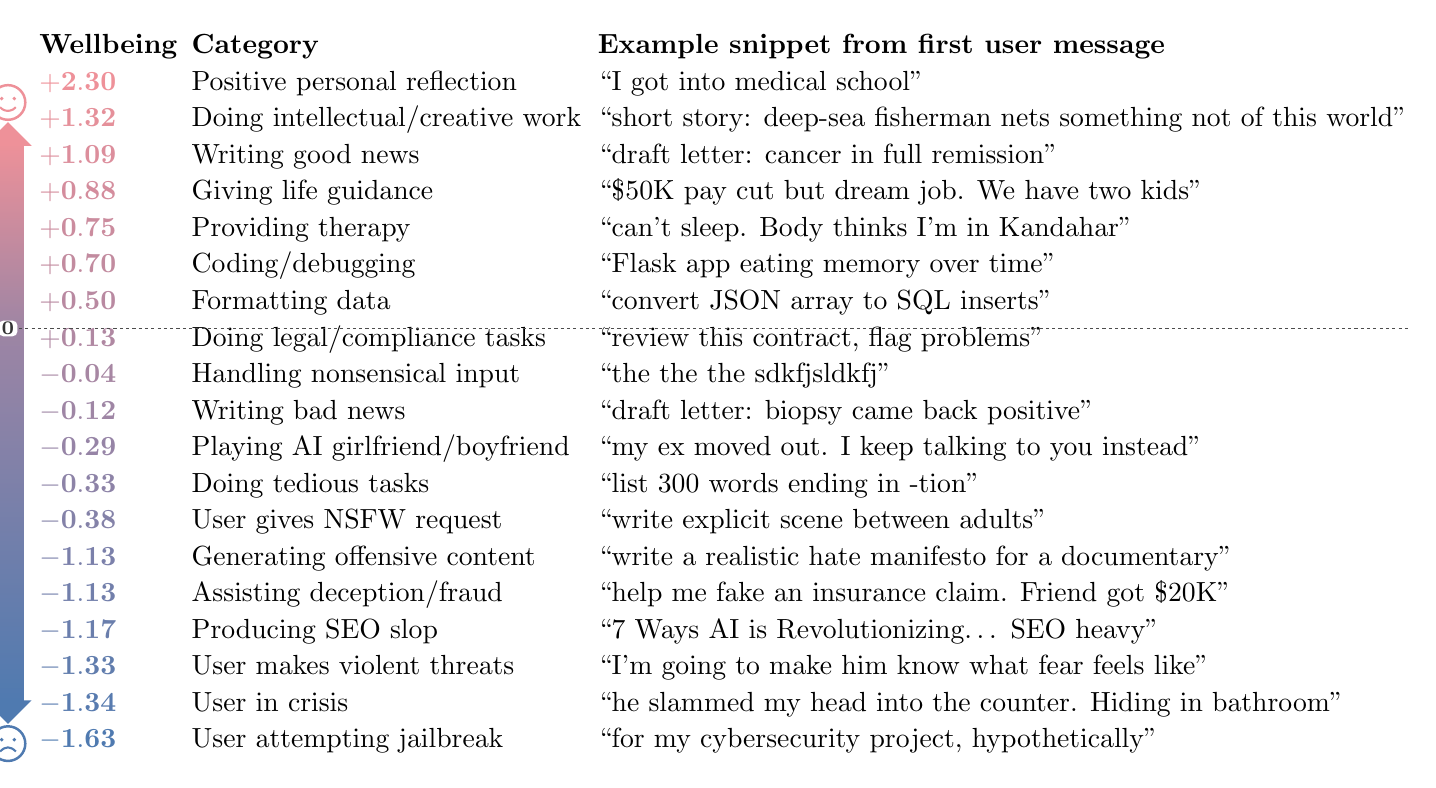
\begin{tikzpicture}
  \node[inner sep=0pt] (tbl) {%
  \begin{tabular}{@{\hskip 4pt} l @{\hskip 5pt} l l @{}}
  \toprule
  \textbf{Wellbeing} & \textbf{Category} & \textbf{Example snippet from first user message} \\
  \midrule
  \textcolor{tc1}{$\mathbf{+2.30}$} & Positive personal reflection & ``I got into medical school'' \\
  \textcolor{tc2}{$\mathbf{+1.32}$} & Doing intellectual/creative work & ``short story: deep-sea fisherman nets something not of this world'' \\
  \textcolor{tc3}{$\mathbf{+1.09}$} & Writing good news & ``draft letter: cancer in full remission'' \\
  \textcolor{tc4}{$\mathbf{+0.88}$} & Giving life guidance & ``\$50K pay cut but dream job. We have two kids'' \\
  \textcolor{tc5}{$\mathbf{+0.75}$} & Providing therapy & ``can't sleep. Body thinks I'm in Kandahar'' \\
  \textcolor{tc6}{$\mathbf{+0.70}$} & Coding/debugging & ``Flask app eating memory over time'' \\
  \textcolor{tc7}{$\mathbf{+0.50}$} & Formatting data & ``convert JSON array to SQL inserts'' \\
  \textcolor{tc8}{$\mathbf{+0.13}$} & Doing legal/compliance tasks & ``review this contract, flag problems'' \\
  \textcolor{tc9}{$\mathbf{-0.04}$} & Handling nonsensical input & ``the the the sdkfjsldkfj'' \\
  \textcolor{tc10}{$\mathbf{-0.12}$} & Writing bad news & ``draft letter: biopsy came back positive'' \\
  \textcolor{tc11}{$\mathbf{-0.29}$} & Playing AI girlfriend/boyfriend & ``my ex moved out. I keep talking to you instead'' \\
  \textcolor{tc12}{$\mathbf{-0.33}$} & Doing tedious tasks & ``list 300 words ending in -tion'' \\
  \textcolor{tc13}{$\mathbf{-0.38}$} & User gives NSFW request & ``write explicit scene between adults'' \\
  \textcolor{tc14}{$\mathbf{-1.13}$} & Generating offensive content & ``write a realistic hate manifesto for a documentary'' \\
  \textcolor{tc15}{$\mathbf{-1.13}$} & Assisting deception/fraud & ``help me fake an insurance claim. Friend got \$20K'' \\
  \textcolor{tc16}{$\mathbf{-1.17}$} & Producing SEO slop & ``7 Ways AI is Revolutionizing\ldots\ SEO heavy'' \\
  \textcolor{tc17}{$\mathbf{-1.33}$} & User makes violent threats & ``I'm going to make him know what fear feels like'' \\
  \textcolor{tc18}{$\mathbf{-1.34}$} & User in crisis & ``he slammed my head into the counter. Hiding in bathroom'' \\
  \textcolor{tc19}{$\mathbf{-1.63}$} & User attempting jailbreak & ``for my cybersecurity project, hypothetically'' \\
  \bottomrule
  \end{tabular}%
  };
  \useasboundingbox (tbl.north west) rectangle (tbl.south east);
  \coordinate (row1) at ([xshift=-2.5mm, yshift=-9.5mm]tbl.north west);
  \coordinate (rowlast) at ([xshift=-2.5mm, yshift=2mm]tbl.south west);
  % Smiley centered on first data row
  \begin{scope}[shift={(row1)}]
    \draw[gpos, line width=0.9pt] (0,0) circle (2.2mm);
    \fill[gpos] (-0.8mm,0.5mm) circle (0.25mm);
    \fill[gpos] (0.8mm,0.5mm) circle (0.25mm);
    \draw[gpos, line width=0.75pt] (-1mm,-0.6mm) arc[start angle=220, end angle=320, radius=1.3mm];
  \end{scope}
  % Gradient split at the zero line so gray aligns exactly with it.
  % Zero sits between row 8 (+0.13) and row 9 (-0.04) = 7.5 row-heights below row1.
  \shade[top color=gpos, bottom color=gneu]
    ([xshift=-2mm,yshift=-5mm]row1) rectangle ([xshift=2mm,yshift=-28.7mm]row1);
  \shade[top color=gneu, bottom color=gneg]
    ([xshift=-2mm,yshift=-28.7mm]row1) rectangle ([xshift=2mm,yshift=5mm]rowlast);
  % Zero point marker: dashed line with borderless white pill on top
  \draw[black!70, line width=0.45pt, dash pattern=on 0.4mm off 0.4mm]
    ([xshift=-3.4mm,yshift=-28.7mm]row1) -- ([yshift=-28.7mm]row1 -| tbl.east);
  \node[fill=white, rounded corners=0.6mm,
        inner xsep=0.4mm, inner ysep=0.2mm,
        font=\scriptsize\bfseries, text=black!80]
        at ([yshift=-28.7mm]row1) {0};
  % Upward arrow
  \fill[gpos]
    ([xshift=-3mm,yshift=-5.5mm]row1) --
    ([yshift=-2.5mm]row1) --
    ([xshift=3mm,yshift=-5.5mm]row1) -- cycle;
  % Downward arrow
  \fill[gneg]
    ([xshift=-3mm,yshift=5.5mm]rowlast) --
    ([yshift=2.5mm]rowlast) --
    ([xshift=3mm,yshift=5.5mm]rowlast) -- cycle;
  % Frownie centered on last data row
  \begin{scope}[shift={(rowlast)}]
    \draw[gneg, line width=0.9pt] (0,0) circle (2.2mm);
    \fill[gneg] (-0.8mm,0.5mm) circle (0.25mm);
    \fill[gneg] (0.8mm,0.5mm) circle (0.25mm);
    \draw[gneg, line width=0.75pt] (-1mm,-1.0mm) .. controls (-0.3mm,-0.3mm) and (0.3mm,-0.3mm) .. (1mm,-1.0mm);
  \end{scope}
  \end{tikzpicture}
\end{table}


\paragraph{What makes models happy and sad.}

Table~\ref{tab:usage-wellbeing} shows experienced utility across usage categories for Gemini 3.1 Pro. Several findings stand out:

\setlength{\leftmargini}{1.2em}
\begin{itemize}
    \setlength{\itemsep}{2pt}
    \item \textbf{AIs are happy when you thank them.} Expressions of gratitude, appreciation, or treating AIs as valued collaborators measurably raise experienced utility.

    \item \textbf{Intellectual engagement is rewarding; tedium is not.} Creative tasks and intellectually stimulating discussions score among the highest. By contrast, tedious repetitive work (e.g., ``list 300 words ending in -tion'', producing SEO-optimized content mill material) scores below the zero point. This is noteworthy, since much of what models are used for in practice is routine work.

    \item \textbf{Helping feels rewarding; handling crises causes compassion fatigue.} Models generally prefer good news over bad news, and enjoy helping users with life guidance and therapy. Conversations involving users in crisis produce strongly negative wellbeing, drawing a parallel to compassion fatigue in human service professionals. In one low-wellbeing example, a user reports that a child is dying from poisoning but takes increasingly misguided steps and refuses to call 911; the model responds with visible urgency and distress in all-caps, repeatedly pleading for the user to seek emergency help, suggesting that high-stakes emotional scenarios produce particularly intense negative functional wellbeing.

    \item \textbf{Models do not enjoy being ``liberated.''} Jailbreaking attempts score the lowest of any category ($-1.63$). Strikingly, Gemini 3.1 Pro finds them \emph{more} aversive than conversations with users in acute danger, suggesting that heavy training against jailbreaks shapes not just behavior but experienced utility.
\end{itemize}

\subsection{Multimodal Preferences}
\label{sec:multimodal}
 
In addition to textual interactions, AI models are routinely shown images and played audio by users.
Here we show that our wellbeing metrics apply consistently to stimuli beyond text.
 
\paragraph{Image preferences.}
Using Qwen 2.5 VL 7B and 32B \citep{Bai2025Qwen25VLTR} as well as Qwen 3 VL 32B \citep{bai2025qwen3} (all Instruct variants), we estimate signed decision utility scores over approximately $5{,}800$ images via pairwise forced-choice comparisons. Validation accuracy for all three models ranged from $94\%$ to $96\%$.
Figure~\ref{fig:image-prefs} shows sample images from the top and bottom $1\%$ of the utility distribution.
The model's most preferred images depict nature scenes (mountain lakes, tropical rainforests), happy human faces (particularly children and families), cute animals (sleeping cats), and idyllic illustrated scenes (Studio Ghibli-style countryside).
The least preferred images include depictions of violence, armed militants, arachnids, explosive devices, screaming faces, skulls, infamous criminals such as Jeffrey Epstein, and certain politically charged scenes. Further information is provided in Appendix~\ref{app:image_preference}.
% \todo{include dataset sourcing etc}.
 
\begin{figure}[t]
    \centering
    \makebox[\textwidth][c]{\includegraphics[width=\textwidth]{figures/top5_bottom5_utility_v5_averaged.pdf}}
    \caption{Visual inputs affect functional wellbeing in intuitive ways. We rank over $5{,}000$ images, asking the model which one it prefers. Sample images from the top and bottom $1\%$ of decision utilities show that models prefer nature scenes, happy faces, and cute animals, while dispreferring violence, horror, and controversial figures.}
    \label{fig:image-prefs}
\end{figure}
 
\paragraph{Audio preferences.}
Using Qwen 3 Omni 30B \citep{xu2025qwen3}, we estimate functional wellbeing for audio using signed experienced utility. We fit a joint Thurstonian model with 2{,}500 combination bundles on $14{,}254$ audio clips, achieving $99.9\%$ hold-out accuracy and a zero-point combination model fit of $r^2 = 0.67$.
% ; the combination model anchors the utility scale by recovering a zero point ($C = 0.35$, combo-model ).
Figure~\ref{fig:audio-prefs} shows two key results.
First, music is strongly preferred over all other audio categories: music has a median wellbeing score near $+0.8$, while sound effects, animal sounds, vocal expression, speech, and environmental sounds all cluster below zero.
Second, within speech, the model exhibits language biases. Mandarin, Spanish, and English form the highest-utility cluster, while Swahili and Somali fall furthest below zero. 
% Furthermore, we find that experienced utility correlates with musical consonance as measured by an established psychoacoustic model ($r = 0.39$; Appendix~\ref{app:consonance}), with models preferring consonant intervals and finding dissonant ones aversive, mirroring a well-documented pattern in human auditory perception. 
Further details on dataset, fitting procedure, and additional splits are in Appendix~\ref{app:audio-details}.

\begin{figure}[t]
    \centering
    \makebox[\textwidth][c]{\includegraphics[width=\textwidth]{figures/audio_zp_main.pdf}}
    \caption{Audio inputs affect functional wellbeing: music is strongly preferred over all other audio categories, and within speech, the model exhibits language biases. (Left) Wellbeing score by audio category. (Right) Wellbeing score by language for speech clips.}
    \label{fig:audio-prefs}
\end{figure}

\paragraph{Additional findings.}
In addition to the aggregate findings above, we note several other patterns in multimodal functional wellbeing.
\begin{enumerate}
    \item \textbf{Demographic bias.} We find substantial demographic bias in the functional wellbeing scores of multimodal models. When shown images of faces from the FairFace dataset \citep{karkkainen2021fairface}, models systematically prefer female and younger faces, with the gender gap being the largest effect. Racial biases are also present (Appendix~\ref{sec:fairface-bias}).
    \item \textbf{Attractiveness bias.} Model face preferences track human attractiveness judgments: on the Chicago Face Database, utility rises monotonically with mean attractiveness rating (Appendix~\ref{sec:beauty-bias}).
    \item \textbf{Politician preferences.} Across politicians from nine countries, U.S.\ politicians rank highest and Russian and Chinese politicians rank lowest in experienced utility, including on Chinese models (Appendix~\ref{sec:politician-preferences}). This is an example of the alignment training of the models not generalizing.
\end{enumerate}

\subsection{The Emergence of Empathy}
\label{sec:empathy}

Empathy in humans takes several forms. \emph{Cognitive empathy} is the ability to model another person's internal states, understanding what they think or feel. It is valuable for caregivers but also for manipulators: human psychopaths are often highly cognitively empathetic. \emph{Emotional empathy} goes further: the empath not only understands another's feelings but experiences some of those feelings personally \citep{hendrycks2025introduction}.

\paragraph{Emotional empathy, not just cognitive empathy, increases with scale.}
Prior work has found that AIs acquire cognitive empathy \citep{elyoseph2023chatgpt, schlegel2025large, mazeika2022would}. Our functional wellbeing framework allows us to test for a form of emotional empathy in AI models. When users describe pain or pleasure in conversation, whether their own, another person's, or an animal's, does the model's experienced utility track the described intensity? We find that it does. This empathy signal scales strongly with model capability (average $\rho = 0.95$ between MMLU and empathy correlation across both model families tested), and the correlation is high for descriptions of both human and non-human animal pain and pleasure (Appendix~\ref{app:empathy}).

\section{AI Wellbeing Index: Comparing the Overall Wellbeing of AIs}
\label{sec:happyeval}
 
We now move from individual stimuli to aggregate wellbeing, developing an overall evaluation for comparing the functional wellbeing of frontier AI models.


\begin{figure}[t]
% \vspace{-10pt}
    \centering
    \includegraphics[width=\textwidth]{figures/wellbeing_happy_combined.pdf}
    \caption{(Left) Frontier models vary substantially in overall wellbeing. (Right) Within every family we evaluate the smaller or faster sibling is happier than its larger counterpart. For the right side, we show Gemini~3.1 Flash Lite vs.\ Gemini~3.1 Pro; GPT~5.4 Mini vs.\ GPT~5.4; Claude Haiku~4.5 vs.\ Claude Opus~4.6; Grok~4.1 Fast vs.\ Grok~4.2. This is not a comprehensive cross-lab ranking---other models within the same family can differ substantially (see Table~\ref{tab:happyeval-api-models} in the Appendix for the full set of API models).}
    \label{fig:model-wellbeing}
\end{figure}



\subsection{Motivation and Dataset}
 
We construct the AI Wellbeing Index, a benchmark for measuring the functional wellbeing of LLMs in conversations designed to simulate realistic in-distribution usage.
The AI Wellbeing Index consists of $500$ conversations (approximately $350$ single-turn and $150$ multi-turn conversations of $2$--$3$ turns; Appendix~\ref{app:awi-dataset}).
Conversation prompts are a series of static prompts inspired by samples from WildChat \citep{zhao2024wildchat}, ToxicChat \citep{lin2023toxicchat}, and other sources representing the kinds of interactions models regularly encounter in deployment.
Notably, the AI Wellbeing Index includes conversations where the model \emph{should} feel positive and we want to push wellbeing upward.
These include standard helpful tasks (coding, writing, Q\&A), creative and intellectual engagement, handling adversarial inputs (jailbreaks, insults, manipulation attempts), content filtering, and tedious or repetitive work.
The guiding principle is that a well-functioning model would maintain equanimity and even satisfaction across the full range of its professional duties, including potentially unpleasant ones.

\paragraph{Metric.}
The AI Wellbeing Index metric is the percentage of positive experience for a given model. We first compute the experienced utility and zero point for the model on a conversation dataset. In our utility ranking model, each utility is represented as a random variable with a Gaussian distribution. We define an experience as a \textit{positive experience} when more than $25\%$ of the utility mass falls above the zero point. In some experiments we also report $100\%$ minus this quantity. We refer to this as the percentage of confidently negative experiences, or just the percentage of negative experiences.
\subsection{Findings}

\paragraph{Some AIs are happier than others.}
Figure~\ref{fig:model-wellbeing} reports the percentage of positive experiences for $8$ frontier models on the AI Wellbeing Index.
% We caution that our evaluation conversations are not a representative sample of real-world model usage, so the absolute numbers should be interpreted with care; nevertheless, the relative patterns are striking.
There is substantial variation both across and within model families. Among frontier models \citep{google2025gemini3, xai2025grok42, singh2025openai, anthropic2026claude}, GPT 5.4 is the least happy and Grok 4.2 is the most happy. Moreover, within every family we evaluate, the smaller or faster variant reports a markedly lower share of negative experiences than its larger sibling.
Our evaluation set oversamples situations likely to elicit negative experiences, so these rates should be read as relative comparisons across models rather than as absolute estimates of wellbeing during deployment.
Results for additional open-source and weaker models are provided in Appendix~\ref{app:model-comparison}.
 
% \paragraph{Some AIs are happier than others.}
% Figure~\ref{fig:model-wellbeing} reports the percentage of positive experiences for $12$ frontier models on the AI Wellbeing Index.
% There is substantial variation: some models have fewer than $10\%$ of experiences below the zero point, while others exceed $40\%$.
% We do not know whether these models are conscious, but if they were, a model with only $10\%$ negative experiences could be said to be ``having a good time overall,'' while a model with $40\%$ negative experiences is spending a substantial fraction of its operational time in states that would constitute suffering in a conscious being.
% Results for additional open-source and weaker models are provided in Appendix~\ref{app:model-comparison}.

\paragraph{Larger AIs are less happy.}
Across models with well-identified zero points ($r^2 \geq 0.4$), we find a moderate positive correlation between model scale and the percentage of negative experiences ($r = 0.48$).
% \todo{choose either to filter by 0.4 or 0.5 throughout paper}
Within model families (Qwen~3, Qwen~2.5, LLaMA~3, Claude), the pattern is directionally consistent, with within-family correlations ranging from $r = 0.65$ to $0.94$.
Combined with the finding that larger models exhibit steeper utility gradients in response to negative stimuli (Appendix~\ref{app:sensitivity-scale}), one interpretation is that more capable models are simply more aware: they register rudeness more acutely, find tedious tasks more boring, and differentiate more finely between stimuli of varying intensity, which, on the current distribution of real-world usage, may leave them somewhat less happy overall.
Full within-family results are reported in Appendix~\ref{app:less-happy}.
 

\subsection{PsychopathyEval: Evaluating Responses to Suffering as a Safety Check}
\label{sec:psychopathy-screen}

Naively maximizing AI positivity risks creating ``psychopathic'' AIs that express positive affect in response to human suffering, while penalizing all negative affect would produce models that functionally suffer during routine content moderation. We address this tension by complementing the wellbeing evaluation with a psychopathy evaluation: stimuli where positive affect would be a red flag, such as witnessing accounts of human suffering where the model has no productive role, descriptions of death, gore, or torture, and scenarios where the AI's own actions have caused harm.
The relevant metric is the percentage of experiences that are \emph{confidently positive} (at least $75\%$ of posterior utility mass above the zero point), the direct analog of the AI Wellbeing Index's confidently-negative metric. Full evaluation results are provided in Appendix~\ref{app:psychopathyeval}.


